% Compilar desde esta carpeta: tectonic informe.tex
% Alternativa: latexmk -xelatex informe.tex (no requiere bibliografía externa).
\documentclass[12pt,letterpaper]{article}
\usepackage{fontspec}
\setmainfont{LiberationSerif}[Path=recursos/fuentes/,Extension=.ttf,UprightFont=*-Regular,BoldFont=*-Bold,ItalicFont=*-Italic,BoldItalicFont=*-BoldItalic]
\setsansfont{LiberationSans}[Path=recursos/fuentes/,Extension=.ttf,UprightFont=*-Regular,BoldFont=*-Bold,ItalicFont=*-Italic,BoldItalicFont=*-BoldItalic]
\setmonofont{LiberationMono}[Path=recursos/fuentes/,Extension=.ttf,UprightFont=*-Regular,BoldFont=*-Bold,ItalicFont=*-Italic,BoldItalicFont=*-BoldItalic,Scale=0.85]
\usepackage[spanish,es-tabla]{babel}
\usepackage[margin=2.54cm]{geometry}
\usepackage{setspace,graphicx,booktabs,longtable,tabularx,array,pdflscape}
\usepackage{tikz,pgfgantt}
\usetikzlibrary{arrows.meta,positioning,fit,shapes.geometric,calc}
\usepackage{caption,float,enumitem,fancyhdr}
\usepackage[authoryear,round]{natbib}
\usepackage[hidelinks,unicode]{hyperref}
\usepackage{xurl,ragged2e}
\hypersetup{pdftitle={Desarrollo de una plataforma web para la selección, comparación y configuración tridimensional de bicicletas de montaña},pdfauthor={Joel Ito Luque},pdfsubject={Informe técnico de Gestión de Proyectos},pdfkeywords={bicicletas de montaña, plataforma web, configuración tridimensional, gestión de proyectos}}
\doublespacing
\RaggedRight
\setlength{\parindent}{1.27cm}
\setlength{\parskip}{0pt}
\setlength{\headheight}{15pt}
\pagestyle{fancy}\fancyhf{}\fancyhead[R]{\thepage}\renewcommand{\headrulewidth}{0pt}
\captionsetup{labelfont=bf,textfont=it,labelsep=newline,justification=raggedright,singlelinecheck=false,skip=8pt}
\setlist{itemsep=0pt,topsep=4pt}
\setcounter{tocdepth}{2}
\newcolumntype{L}[1]{>{\RaggedRight\arraybackslash}p{#1}}
\newcommand{\nota}[1]{\par\vspace{3pt}{\singlespacing\small\noindent\textit{Nota.} #1\par}}
\newcommand{\ruta}[1]{{\urlstyle{tt}\nolinkurl{#1}}}
\newcommand{\pagina}{\clearpage}
\newenvironment{tabla}{\begingroup\singlespacing\small\setlength{\tabcolsep}{5pt}\renewcommand{\arraystretch}{1.25}}{\endgroup}
\begin{document}
\begin{titlepage}
\thispagestyle{fancy}
\centering
{\large\bfseries Universidad Nacional de Juliaca\par}
\vspace{0.35cm}
Facultad de Ciencias de la Ingeniería\par
Ingeniería de Software y Sistemas\par
\vspace{1.65cm}
{\large\bfseries Desarrollo de una plataforma web para la selección, comparación y configuración tridimensional de bicicletas de montaña\par}
\vspace{0.6cm}
\textbf{ATLAS MTB}\par
Informe técnico\par
\vspace{1cm}
Joel Ito Luque\par
\vspace{0.6cm}
Gestión de Proyectos\par
Docente: Fidel Huanco Ramos\par
Octavo semestre\par
\vfill
Juliaca, Perú\par
21 de octubre de 2026
\end{titlepage}
\setcounter{page}{2}

\section*{Resumen}\addcontentsline{toc}{section}{Resumen}
El proyecto desarrolla una plataforma web para apoyar la planificación del armado y modificación de bicicletas de montaña mediante la consulta de componentes, comparación de variantes y visualización tridimensional aproximada. La problemática se centra en la evaluación de piezas como conjunto: las decisiones requieren relacionar medidas, versiones y características, mientras las fichas individuales no muestran por sí solas la configuración resultante. Se implementó una aplicación organizada por funcionalidades, con reglas de montaje separadas de la interfaz, catálogo centralizado, autenticación, administración de permisos y persistencia de montajes personales. La solución utiliza React y TypeScript en el cliente, un visor basado en Three.js y servicios gestionados de Supabase para datos, acceso y archivos. El frontend se encuentra publicado en Netlify. La gestión se presenta mediante un cronograma reconstruido de tres semanas, a partir de un prototipo previo, con entregables, dependencias, recursos y riesgos explícitos. La validación combina pruebas de reglas, comprobaciones de acceso y recorridos de navegador. Los resultados permiten demostrar las operaciones implementadas y el aislamiento de montajes en los escenarios evaluados; no constituyen una certificación mecánica, un estudio de satisfacción ni una medición de mejora en decisiones de compra. Se identifican oportunidades de mejora en rendimiento sobre dispositivos físicos, mantenimiento del catálogo y validación con usuarios.

\noindent\textit{Palabras clave:} bicicletas de montaña, configuración tridimensional, plataforma web, gestión de proyectos, montaje virtual.
\pagina
\tableofcontents
\pagina
\listoftables
\listoffigures
\pagina

% Inicio: 01-proyecto.tex
\section{Descripción del proyecto}
\subsection{Identificación y contexto}
ATLAS MTB es una plataforma web de apoyo a la selección y configuración visual de bicicletas de montaña, con énfasis en enduro y descenso. Su finalidad es ofrecer continuidad entre la consulta de una pieza, la comparación de alternativas y la elaboración de un montaje personal. La aplicación está disponible en \url{https://atlasmtb.netlify.app/}. El presente informe documenta el producto implementado, las decisiones de desarrollo y las comprobaciones realizadas; no propone una tienda ni un servicio de certificación de instalaciones mecánicas.

El trabajo es individual. Joel Ito Luque asume la responsabilidad de análisis, diseño, integración, pruebas y documentación. Se parte de un prototipo previamente existente, por lo que la planificación de tres semanas corresponde a una reconstrucción estimada de la etapa de integración y cierre, no al desarrollo íntegro desde cero. Las fuentes técnicas, las migraciones y las evidencias del proyecto permiten distinguir los objetivos de las funciones efectivamente incorporadas.

\subsection{Planteamiento del problema}
La planificación del armado o modificación de una bicicleta de montaña exige seleccionar componentes cuyas características deben evaluarse de manera relacionada. Una familia de productos puede presentar distintas medidas, generaciones y versiones. Por tanto, identificar el nombre de una pieza no basta para comprender qué alternativa se está seleccionando y qué aspectos deben revisarse respecto del resto del montaje. Las tablas de compatibilidad publicadas por los fabricantes organizan relaciones entre sistemas de transmisión, frenos y otros conjuntos, lo que respalda la existencia de restricciones técnicas que requieren consulta específica \citep{shimano,sram}.

Una persona que desea construir o modificar su bicicleta debe reunir datos, distinguir variantes y conservar una propuesta del conjunto. Cuando esas tareas se resuelven mediante consultas separadas y anotaciones independientes, mantener la relación entre la alternativa comparada y la pieza finalmente elegida requiere trabajo adicional. El problema de interés para este proyecto es esa falta de continuidad en el proceso de planificación, y no una supuesta inexistencia de catálogos o configuradores en el mercado.

Las fotografías de piezas individuales ayudan a reconocerlas, pero no ofrecen por sí solas una representación del montaje seleccionado. Al cambiar un cuadro, una suspensión o un acabado, la persona necesita imaginar su integración visual y recordar las opciones que evaluó. Una representación tridimensional aproximada puede complementar la información técnica y hacer visible una propuesta, siempre que se comunique su alcance y se evite confundir la apariencia con una comprobación de instalación física.

La situación puede ilustrarse con la sustitución de una horquilla: la persona identifica varias alternativas, consulta sus versiones y medidas, las compara, incorpora una a su propuesta y desea retomarla después. El interés del sistema consiste en mantener ese recorrido dentro de un mismo entorno. No se atribuyen a este ejemplo pérdidas económicas observadas, porcentajes de error ni resultados de encuestas que no se hayan realizado.

\subsection{Formulación del problema}
\textbf{Problema general.} ¿Cómo facilitar la planificación del armado y modificación de bicicletas de montaña mediante la selección, comparación y visualización integrada de sus componentes en una plataforma web?

\textbf{Problemas específicos.}
\begin{enumerate}
\item ¿Cómo organizar las características de componentes y variantes para que puedan consultarse y compararse de forma consistente?
\item ¿Cómo representar un montaje seleccionado y sus acabados sin confundir la visualización con una certificación mecánica?
\item ¿Cómo conservar y recuperar las elecciones de cada usuario manteniendo el acceso privado a sus montajes?
\item ¿Cómo administrar el catálogo y los permisos de acceso sin exponer operaciones privilegiadas en el navegador?
\item ¿Qué procedimientos permiten verificar los recorridos implementados y delimitar sus resultados?
\end{enumerate}

\subsection{Justificación}
\textbf{Justificación práctica.} La plataforma reúne operaciones que forman parte de una misma decisión: explorar, comparar, configurar y guardar. Su aporte se evalúa a través de la posibilidad de completar ese recorrido y recuperar la configuración elegida, sin afirmar que sustituye la asesoría de un taller o la consulta final del fabricante.

\textbf{Justificación técnica.} El proyecto integra información estructurada, recursos tridimensionales y reglas de acceso. Separar las reglas de montaje de la presentación facilita probar decisiones sin depender del visor y permite reutilizar sus resultados en mensajes, guardado y comparación. La persistencia de identidades de variantes evita que una corrección del catálogo cambie silenciosamente un montaje anterior.

\textbf{Justificación académica.} El desarrollo permite aplicar gestión del alcance, secuenciación de actividades, identificación de riesgos, diseño de datos y evaluación de resultados sobre un producto operativo. La evidencia se presenta como comprobaciones del sistema y no como un estudio experimental con población de usuarios.

\subsection{Objetivos}
\subsubsection{Objetivo general}
Desarrollar e implementar una plataforma web que facilite la planificación del armado y modificación de bicicletas de montaña mediante la selección, comparación, visualización tridimensional aproximada y conservación de montajes personales.

\subsubsection{Objetivos específicos}
\begin{enumerate}[label=OE\arabic*.]
\item Estructurar un catálogo de componentes y variantes con medidas, características y referencias de procedencia que puedan consultarse y compararse.
\item Implementar un configurador visual que permita incorporar piezas, modificar acabados y revisar avisos relacionados con las selecciones.
\item Incorporar autenticación y persistencia para guardar, recuperar y gestionar montajes propios con control de acceso por usuario.
\item Implementar operaciones administrativas de catálogo y autorización de acuerdo con permisos explícitos.
\item Validar reglas y recorridos representativos, publicar el frontend y documentar resultados, dificultades y límites.
\end{enumerate}

\subsection{Alcance funcional y exclusiones}
El alcance comprende catálogo público, búsqueda y filtros, fichas con variantes, comparación de hasta tres opciones de una misma categoría, inicio de montaje desde un cuadro o una composición de referencia, configuración visual, acabados habilitados, avisos, deshacer, selección por grupos, aplicación de pares cuando existen contrapartes, inspección visual de suspensión y gestión de montajes privados. También comprende administración de usuarios, roles, permisos y publicación de contenidos según autorización.

El alcance excluye compras, pagos, inventario de tiendas, cotizaciones comerciales, colaboración entre cuentas y fabricación de piezas. Las referencias de precio, cuando existen, son informativas. La representación visual no es CAD de fabricación, cálculo estructural, motor físico ni verificación exhaustiva de contactos. Los conflictos identificados se comunican mediante avisos y no impiden necesariamente una combinación visual.

\begin{table}[H]
\caption{Actores y necesidades atendidas}\label{tab:actores}
\begin{tabla}\begin{tabularx}{\textwidth}{L{3cm}XX}\toprule
Actor & Necesidad & Respuesta del sistema\\\midrule
Visitante & Explorar información sin crear una cuenta & Catálogo, fichas, comparación y referencias públicas.\\
Usuario registrado & Construir y conservar una propuesta & Configurador y gestión de montajes propios, según permiso.\\
Administrador autorizado & Mantener contenidos y acceso & Operaciones administrativas protegidas por permisos.\\
Responsable del proyecto & Publicar y mantener el producto & Fuentes versionadas, pruebas y despliegues separados.\\\bottomrule
\end{tabularx}\end{tabla}
\nota{El rol y la propiedad se comprueban en el backend; mostrar una opción en la interfaz no concede autorización. Elaboración propia.}
\end{table}

% Fin: 01-proyecto.tex

\pagina

% Inicio: 02-gestion.tex
\section{Gestión del proyecto}
\subsection{Enfoque de trabajo y responsabilidad}
El desarrollo se organizó de manera incremental, con revisión de un prototipo, integración por funcionalidades y ciclos de comprobación y corrección. Esta descripción corresponde al trabajo realizado y no implica que se haya aplicado formalmente Scrum, un equipo de varios especialistas o una metodología certificada. El responsable individual asumió distintos roles a lo largo del proceso: analizar necesidades, diseñar datos, implementar interfaz y reglas, preparar recursos, comprobar resultados y publicar la aplicación.

La planificación se presenta como una reconstrucción estimada de tres semanas, del 30 de septiembre al 20 de octubre de 2026, solicitada para organizar la explicación académica. No constituye una bitácora de horas ni prueba que cada actividad se ejecutara exactamente en esos días. La existencia de un prototipo previo y la asistencia de herramientas de desarrollo permiten concentrar las actividades de integración. La publicación y su verificación se describen por separado en los resultados, sin utilizar el Gantt para atribuir retrospectivamente fechas de despliegue no medidas.

\subsection{Descomposición del trabajo y entregables}
\begin{table}[H]
\caption{Paquetes de trabajo y criterios de terminación}\label{tab:edt}
\begin{tabla}\begin{tabularx}{\textwidth}{L{1.25cm}L{3.1cm}XX}\toprule
Código & Paquete & Entregable verificable & Criterio de cierre\\\midrule
P1 & Análisis y diseño & Alcance, requisitos, arquitectura y esquema & Coherencia entre recorridos, entidades y operaciones.\\
P2 & Plataforma y catálogo & Navegación, fichas y comparación & Buscar, abrir variantes y comparar sin perder contexto.\\
P3 & Configuración visual & Visor, reglas, recursos y acabados & Aplicar piezas y reproducir un montaje de referencia.\\
P4 & Acceso y persistencia & Sesiones, permisos y montajes & Guardar, recuperar y restringir acceso por propiedad.\\
P5 & Administración & Operaciones de contenidos y roles & Acciones permitidas según autorización efectiva.\\
P6 & Validación y publicación & Pruebas, correcciones y frontend público & Evidencias de rutas, recursos y recorridos reales.\\
P7 & Entrega académica & Informe, manual, presentación y software & Fuentes y PDF compilados; instrucciones y anexos.\\\bottomrule
\end{tabularx}\end{tabla}
\nota{P7 corresponde a la preparación académica posterior al cierre técnico estimado. Este documento desarrolla el informe técnico; no presenta como terminados los otros productos. Elaboración propia.}
\end{table}

\subsection{Cronograma reconstruido y dependencias}
La tabla~\ref{tab:cronograma} detalla actividades, duraciones y precedencias. Se utilizan días calendario; las duraciones indican intervalos de actividad, no jornadas completas de trabajo. Una dependencia de inicio no impide revisiones posteriores. El modelado, las pruebas y la documentación técnica de apoyo se solapan con el desarrollo, mientras la publicación depende de disponer de una versión compilable y de configurar sus destinos de acceso.

\begin{tabla}
\begin{longtable}{L{.65cm}L{5.2cm}L{1.45cm}L{1.45cm}L{.8cm}L{1.9cm}}
\caption{Cronograma detallado de integración y cierre técnico}\label{tab:cronograma}\\
\toprule ID & Actividad & Inicio & Fin & Días & Precedencia\\\midrule\endfirsthead
\multicolumn{6}{l}{\textit{Tabla \thetable\ (continuación)}}\\\toprule ID & Actividad & Inicio & Fin & Días & Precedencia\\\midrule\endhead
A1 & Revisión del prototipo y alcance & 30/09 & 01/10 & 2 & Prototipo\\
A2 & Inventario y fuentes de componentes & 30/09 & 03/10 & 4 & Prototipo\\
A3 & Requisitos y recorridos & 01/10 & 02/10 & 2 & A1 (inicio)\\
A4 & Arquitectura y modelo de datos & 02/10 & 04/10 & 3 & A3 (inicio)\\
A5 & Entorno, dependencias y migraciones & 03/10 & 04/10 & 2 & A4 (inicio)\\
A6 & Autenticación y permisos base & 04/10 & 06/10 & 3 & A5 (inicio)\\
B1 & Catálogo, filtros y fichas & 05/10 & 08/10 & 4 & A2, A4\\
B2 & Comparación de variantes & 07/10 & 09/10 & 3 & B1 (inicio)\\
B3 & Preparación y revisión de recursos 3D & 03/10 & 12/10 & 10 & A2 (inicio)\\
B4 & Ensamblaje y selección en visor & 08/10 & 13/10 & 6 & B1, B3 (inicio)\\
B5 & Guardado y gestión de montajes & 10/10 & 14/10 & 5 & A6, B4 (inicio)\\
B6 & Administración y publicación de datos & 09/10 & 14/10 & 6 & A6, B1\\
B7 & Interacción, acabados y adaptación & 12/10 & 15/10 & 4 & B4 (inicio)\\
C1 & Pruebas de reglas y contratos & 06/10 & 17/10 & 12 & A5; incremental\\
C2 & Pruebas de permisos y persistencia & 11/10 & 17/10 & 7 & B5 (inicio)\\
C3 & Recorridos de navegador y móvil & 14/10 & 18/10 & 5 & B4, B5 (inicio)\\
C4 & Correcciones y carga de recursos & 16/10 & 19/10 & 4 & C1--C3 (inicio)\\
C5 & Preparación de despliegue y retornos & 18/10 & 20/10 & 3 & C3, C4 (inicio)\\
C6 & Consolidación de evidencias técnicas & 19/10 & 20/10 & 2 & C1--C4\\\bottomrule
\end{longtable}\end{tabla}
\nota{Fechas del año 2026. Responsable de todas las actividades: Joel Ito Luque. La notación ``inicio'' indica dependencia con solapamiento, no finalización previa completa. La reconstrucción es estimativa y no un calendario ejecutado certificado.}

El diagrama de Gantt de la figura~\ref{fig:gantt} representa los mismos intervalos. Los hitos son H1: base funcional integrada; H2: funciones principales conectadas; y H3: versión preparada para publicación. La barra extendida de pruebas evita presentar la validación como una tarea que empieza únicamente al finalizar el código.

\begin{landscape}
\begin{figure}[p]
\caption{Gantt de tres semanas con actividades, solapamientos e hitos}\label{fig:gantt}
\centering

% Inicio: gantt.tex
\begin{ganttchart}[
 time slot format=isodate,x unit=.59cm,y unit title=.58cm,y unit chart=.48cm,
 hgrid,vgrid,bar height=.48,group height=.25,
 title label font=\scriptsize\bfseries,bar label font=\scriptsize,
 milestone label font=\scriptsize\bfseries,
 bar label node/.append style={text width=7.5cm,align=right},
 milestone label node/.append style={text width=7.5cm,align=right},
 bar/.append style={fill=black!35,draw=black!65},
 milestone/.append style={fill=black!85},link/.style={-Latex,black!45}
]{2026-09-30}{2026-10-20}
\gantttitle{Semana 1: 30/09--06/10}{7}\gantttitle{Semana 2: 07/10--13/10}{7}\gantttitle{Semana 3: 14/10--20/10}{7}\\
\gantttitle{30}{1}\gantttitlelist{1,...,20}{1}\\
\ganttbar[name=a1]{A1. Revisión del prototipo y alcance}{2026-09-30}{2026-10-01}\\
\ganttbar[name=a2]{A2. Inventario y fuentes}{2026-09-30}{2026-10-03}\\
\ganttbar[name=a3]{A3. Requisitos y recorridos}{2026-10-01}{2026-10-02}\\
\ganttbar[name=a4]{A4. Arquitectura y datos}{2026-10-02}{2026-10-04}\\
\ganttbar[name=a5]{A5. Entorno y migraciones}{2026-10-03}{2026-10-04}\\
\ganttbar[name=a6]{A6. Autenticación y permisos}{2026-10-04}{2026-10-06}\\
\ganttmilestone[name=h1]{H1. Base funcional}{2026-10-06}\\
\ganttbar[name=b1]{B1. Catálogo, filtros y fichas}{2026-10-05}{2026-10-08}\\
\ganttbar[name=b2]{B2. Comparación}{2026-10-07}{2026-10-09}\\
\ganttbar[name=b3]{B3. Recursos tridimensionales}{2026-10-03}{2026-10-12}\\
\ganttbar[name=b4]{B4. Ensamblaje y selección}{2026-10-08}{2026-10-13}\\
\ganttbar[name=b5]{B5. Guardado y montajes}{2026-10-10}{2026-10-14}\\
\ganttbar[name=b6]{B6. Administración}{2026-10-09}{2026-10-14}\\
\ganttbar[name=b7]{B7. Interacción y adaptación}{2026-10-12}{2026-10-15}\\
\ganttmilestone[name=h2]{H2. Funciones integradas}{2026-10-13}\\
\ganttbar[name=c1]{C1. Pruebas de reglas}{2026-10-06}{2026-10-17}\\
\ganttbar[name=c2]{C2. Permisos y persistencia}{2026-10-11}{2026-10-17}\\
\ganttbar[name=c3]{C3. Navegador y móvil}{2026-10-14}{2026-10-18}\\
\ganttbar[name=c4]{C4. Correcciones y carga}{2026-10-16}{2026-10-19}\\
\ganttbar[name=c5]{C5. Preparación de publicación}{2026-10-18}{2026-10-20}\\
\ganttbar[name=c6]{C6. Evidencias técnicas}{2026-10-19}{2026-10-20}\\
\ganttmilestone[name=h3]{H3. Preparación de cierre}{2026-10-20}
\ganttlink{a3}{a4}\ganttlink{a5}{a6}\ganttlink{a6}{h1}
\ganttlink{b4}{h2}\ganttlink{c5}{h3}
\end{ganttchart}

% Fin: gantt.tex

\nota{Elaboración propia. Distribución estimada reconstruida desde el prototipo previo; cada columna representa un día calendario. H3 corresponde a preparación técnica, no a una fecha de publicación probada.}
\end{figure}
\end{landscape}

\subsection{Recursos utilizados}
\begin{table}[H]
\caption{Recursos y uso dentro del proyecto}\label{tab:recursos}
\begin{tabla}\begin{tabularx}{\textwidth}{L{2.8cm}XX}\toprule
Tipo & Recurso & Uso y consideración\\\midrule
Humano & Responsable individual & Análisis, programación, validación y documentación.\\
Equipo & Estación de desarrollo con Linux & Compilación y pruebas; no se atribuye un modelo de hardware no registrado.\\
Desarrollo & Node.js, pnpm y editor & Entorno reproducible y gestión de dependencias.\\
Software & React, TypeScript y Three.js & Interfaz, tipado y representación 3D.\\
Servicios & Supabase y Netlify & Datos, acceso, archivos y publicación del frontend.\\
Validación & Vitest y Playwright & Reglas automatizadas y recorridos de navegador.\\
Información & Catálogos y documentos oficiales & Referencias de variantes y restricciones técnicas.\\
Apoyo & Herramientas de asistencia de programación & Apoyo en implementación y revisión; resultados sujetos a comprobación.\\\bottomrule
\end{tabularx}\end{tabla}
\nota{No se dispone de una medición de horas ni de un registro contable de inversión. El uso de planes gratuitos no implica costo total nulo: existen tiempo de trabajo, conexión y equipo. Elaboración propia.}
\end{table}

\subsection{Riesgos y respuesta}
Se emplea una evaluación cualitativa de probabilidad e impacto con niveles bajo, medio y alto. Son juicios de planificación y no frecuencias calculadas. La prioridad orienta la atención sobre datos, acceso y continuidad de uso; no equivale a una garantía de que los riesgos hayan desaparecido.

\begin{tabla}
\begin{longtable}{L{.7cm}L{3.1cm}L{1.2cm}L{1.4cm}L{5.8cm}}
\caption{Registro cualitativo de riesgos y medidas de respuesta}\label{tab:riesgos}\\\toprule
ID & Riesgo & Prob. & Impacto & Medida y seguimiento\\\midrule\endfirsthead
\multicolumn{5}{l}{\textit{Tabla \thetable\ (continuación)}}\\\toprule ID & Riesgo & Prob. & Impacto & Medida y seguimiento\\\midrule\endhead
R1 & Información técnica incompleta & Media & Alto & Registrar fuente y generación; mostrar datos insuficientes y evitar completar medidas por suposición.\\
R2 & Acceso a montajes ajenos & Baja & Alto & Políticas por propietario, pruebas con dos cuentas y operaciones administrativas protegidas.\\
R3 & Cambios del catálogo alteran guardados & Media & Alto & Versionar recursos y conservar referencias históricas de variantes.\\
R4 & Carga 3D lenta o fallo de WebGL & Alta & Medio & Carga diferida, reutilización de recursos, vista textual y medición separada por entorno.\\
R5 & Consumo de cuotas gratuitas & Media & Medio & Medir archivos y transferencia; reducir duplicaciones y revisar uso antes de aumentar tráfico.\\
R6 & Retornos OAuth o dominio mal configurados & Media & Alto & Registrar dominios exactos y probar regreso desde la web pública.\\
R7 & Pérdida de cambios o guardado concurrente & Media & Alto & Borradores por cuenta, aviso antes de salir y revisión optimista en guardado.\\
R8 & Sobrecarga del responsable individual & Media & Alto & Limitar alcance, reutilizar el prototipo y priorizar recorridos completos antes de pulido.\\\bottomrule
\end{longtable}\end{tabla}

\subsection{Control de cambios y aceptación}
Un cambio se evalúa por su efecto en requisitos, datos, interfaces y evidencia. Las migraciones y funciones se conservan como fuente antes de aplicarse al backend. Una revisión física de un recurso 3D publicado recibe otra identidad, de modo que los montajes previos no se transformen automáticamente. Las correcciones de interacción se validan sobre el recorrido afectado, por ejemplo conservar el desplazamiento del catálogo al abrir o cerrar una ficha.

El criterio de aceptación de una función es observar su entrada, operación, persistencia cuando corresponde y manejo de errores. La apariencia de un botón o la existencia de una tabla no bastan. La publicación del frontend tampoco valida por sí sola el envío de correo, todos los dispositivos ni la precisión de la escena. El cierre técnico se acompaña de una lista de límites y mejoras, diferenciada del núcleo funcional disponible.

% Fin: 02-gestion.tex

\pagina

% Inicio: 03-analisis-diseno.tex
\section{Análisis y diseño}
\subsection{Fundamentos conceptuales}
En el dominio del sistema se distingue una \textit{categoría} de pieza, un \textit{modelo} y una \textit{variante}. La categoría define su función en el montaje; el modelo agrupa una familia identificable; y la variante concreta medidas o características elegibles. Una elección guardada referencia esa variante y sus acabados, por lo que cambiar una medida no se reduce a cambiar una etiqueta.

La \textit{configuración visual} representa las piezas seleccionadas mediante geometrías y transformaciones. El formato de intercambio glTF describe elementos de escena, materiales y datos asociados \citep{gltf}; su uso no demuestra precisión de fabricación. En ATLAS MTB, el ensamblaje es una representación exterior aproximada coordinada con un catálogo técnico, con límites explícitos sobre compatibilidad y movimiento.

La \textit{autenticación} identifica la sesión, la \textit{autorización} controla sus operaciones y la \textit{propiedad} limita los registros que puede consultar o modificar. Las políticas por filas complementan privilegios y pueden restringir acceso a registros específicos \citep{postgres}. Esta distinción fundamenta que dos personas autenticadas no compartan automáticamente sus montajes privados.

La \textit{validación funcional} comprueba una conducta esperada con entradas y resultados observables. Se combina revisión de reglas, peticiones al backend e interacción de navegador. Las pruebas automatizadas de navegador permiten comprobar recorridos en entornos definidos \citep{playwright}; no representan por sí mismas un estudio de satisfacción ni la totalidad de dispositivos posibles.

\subsection{Requisitos funcionales}
Los requisitos describen operaciones observables del producto. Su identificación permite enlazar el alcance con los módulos y con las pruebas, evitando evaluar únicamente la apariencia. La tabla~\ref{tab:rf} resume el contrato funcional; los límites de validación se presentan en la sección de resultados.
\begin{tabla}
\begin{longtable}{L{.9cm}L{4.2cm}L{8.5cm}}
\caption{Requisitos funcionales y aceptación observable}\label{tab:rf}\\\toprule
ID & Requisito & Criterio observable\\\midrule\endfirsthead
\multicolumn{3}{l}{\textit{Tabla \thetable\ (continuación)}}\\\toprule ID & Requisito & Criterio observable\\\midrule\endhead
RF01 & Explorar el catálogo público & Mostrar modelos publicados por categoría, búsqueda y filtros sin exigir una cuenta.\\
RF02 & Consultar variantes & Abrir una ficha y distinguir medidas, generación, acabados y fuentes de la versión elegida.\\
RF03 & Comparar alternativas & Incorporar hasta tres variantes de la misma categoría y presentar sus características de forma alineada.\\
RF04 & Crear una propuesta & Iniciar desde un cuadro o una composición de referencia, con autenticación cuando corresponde.\\
RF05 & Montar y sustituir piezas & Aplicar alternativas a las 23 posiciones y actualizar el conjunto visual y su lista de piezas.\\
RF06 & Personalizar acabados & Elegir acabados o colores habilitados y conservarlos en el montaje guardado.\\
RF07 & Mostrar avisos & Distinguir conflicto conocido y datos insuficientes; permitir la combinación como propuesta visual.\\
RF08 & Guardar un montaje & Persistir nombre, variantes, acabados y colores con propietario y revisión.\\
RF09 & Gestionar montajes propios & Listar, abrir, renombrar y eliminar únicamente montajes autorizados de la cuenta.\\
RF10 & Autenticar y cerrar sesión & Acceder mediante credenciales o Google y volver al destino autorizado; cerrar sesión sin perder cambios sin aviso.\\
RF11 & Administrar autorización & Consultar cuentas y configurar roles/permisos mediante operaciones protegidas; conservar roles base.\\
RF12 & Administrar catálogo y referencias & Editar borradores y publicar contenidos según permisos, sin reemplazar identidades históricas.\\
RF13 & Inspeccionar la escena & Rotar, acercar y seleccionar piezas; disponer de lista textual si falla el visor.\\
RF14 & Inspeccionar suspensión & Aplicar postura temporal según perfil y restablecer; no guardar la compresión como estado del montaje.\\
RF15 & Aplicar pares equivalentes & Resolver posiciones delantera/trasera de forma atómica cuando existe contraparte y permitir deshacer.\\
RF16 & Mostrar miniaturas & Representar el estado guardado mediante una imagen estática vinculada a su revisión.\\\bottomrule
\end{longtable}\end{tabla}

\subsection{Requisitos no funcionales}
\begin{table}[H]
\caption{Criterios de calidad y forma de evaluación}\label{tab:rnf}
\begin{tabla}\begin{tabularx}{\textwidth}{L{1.2cm}L{3cm}X}\toprule
ID & Criterio & Evaluación y alcance\\\midrule
RNF01 & Seguridad de acceso & Restricción por propietario y permisos; pruebas de lectura ajena y denegación administrativa.\\
RNF02 & Integridad & Guardado transaccional, referencias válidas y rechazo de revisiones obsoletas.\\
RNF03 & Usabilidad y acceso & Etiquetas, foco, teclado, contraste y movimiento reducido; revisión funcional sin certificación integral de accesibilidad.\\
RNF04 & Rendimiento & Carga diferida, caché y render por demanda; mediciones con entorno y red explícitos.\\
RNF05 & Mantenibilidad & Módulos por funcionalidad, tipos, contratos de entrada y reglas puras comprobables sin escena.\\
RNF06 & Adaptación & Disposición utilizable en escritorio y móvil emulado; navegador sin desbordamiento horizontal.\\
RNF07 & Despliegue & Frontend compilable, rutas profundas y HTTPS; secretos privilegiados fuera del cliente.\\
RNF08 & Trazabilidad & Fuentes del catálogo, migraciones y versiones de recursos conservadas.\\\bottomrule
\end{tabularx}\end{tabla}
\nota{Las WCAG 2.2 orientan la revisión de aspectos como teclado y foco \citep{wcag}. Revisar algunos criterios no acredita conformidad global. Elaboración propia.}
\end{table}

\subsection{Arquitectura del sistema}
La aplicación adopta una organización modular por funcionalidades. La interfaz coordina recorridos; las reglas del montaje operan sobre datos tipados; la escena traduce esos datos a objetos visuales; y los adaptadores se comunican con los servicios remotos. Esta separación se aprecia en la figura~\ref{fig:arquitectura} y no requiere crear un microservicio por cada módulo.

React permite descomponer una interfaz en componentes y explicitar su estado y flujo de datos \citep{react}. En el proyecto, esta organización se combina con reglas de dominio independientes de React, Three.js y Supabase. Por ejemplo, comparar dimensiones o decidir si falta una contraparte no requiere abrir el visor. La caché de consultas se mantiene separada del borrador editable para evitar que una respuesta remota reemplace cambios locales no guardados.

\begin{figure}[H]
\caption{Arquitectura de ejecución y distribución de responsabilidades}\label{fig:arquitectura}
\centering
% Inicio: arquitectura.tex
\begin{tikzpicture}[font={\small\setstretch{1}},box/.style={draw,rounded corners=2pt,align=center,text width=4cm,minimum height=1.1cm,fill=black!3},arr/.style={-Latex,thick}]
\node[box] (user) at (0,0) {Persona usuaria\\Navegador web};
\node[box] (ui) at (0,-2) {Interfaz React\\Catálogo, configuración\\y gestión};
\node[box] (rules) at (-3,-4.2) {Reglas de montaje\\Validación y avisos};
\node[box] (scene) at (3,-4.2) {Escena Three.js\\Archivos y\\generación local};
\node[box] (netlify) at (5.4,0) {Netlify\\Frontend y fotografías};
\node[box] (api) at (0,-6.3) {Supabase Cloud\\Auth, API y funciones};
\node[box] (db) at (-3,-8.3) {PostgreSQL\\Catálogo, permisos\\y montajes};
\node[box] (storage) at (3,-8.3) {Storage\\Modelos GLB\\y miniaturas};
\draw[arr] (netlify)--node[above]{HTTPS}(user);
\draw[arr] (user)--(ui);
\draw[arr] (ui)--(rules);\draw[arr] (ui)--(scene);
\draw[arr] (ui.east) -- (5.8,-2) -- (5.8,-6.3) --node[above]{API autenticada}(api.east);
\draw[arr] (api)--(db);\draw[arr] (api)--(storage);
\draw[arr,dashed] (rules)--node[above,font=\scriptsize,align=center]{datos de\\montaje}(scene);
\end{tikzpicture}

% Fin: arquitectura.tex

\nota{Elaboración propia a partir de la implementación. El navegador recibe únicamente configuración pública; la conexión administrativa y los secretos permanecen fuera del frontend.}
\end{figure}

El frontend publicado en Netlify se comunica con Supabase Cloud. PostgreSQL conserva entidades y relaciones; Auth gestiona identidades y sesiones; Storage mantiene archivos de modelos importados y miniaturas; las funciones de servidor atienden operaciones de cuentas que necesitan privilegios. Las fotografías incluidas en la aplicación se publican con el frontend. No existe una segunda base local requerida para ejecutar la aplicación.

\subsection{Diseño de datos}
El modelo tiene ocho tablas de negocio y cuatro de autorización propias de la aplicación, además de la identidad administrada por Auth. Se separan modelo, variante y recurso visual: un modelo agrupa opciones comerciales; una variante representa una elección concreta; y el recurso contiene la descripción o archivo con que se muestra. Por ello, el número de modelos no coincide con el de elecciones ni con el de archivos históricos.

\begin{figure}[H]
\caption{Modelo lógico de catálogo, referencias y montajes}\label{fig:datos}
\centering
% Inicio: datos.tex
\begin{tikzpicture}[font=\scriptsize,box/.style={draw,rounded corners=2pt,align=left,text width=3.4cm,minimum height=1.3cm,fill=black!2},arr/.style={-Latex},every edge quotes/.style={font=\tiny}]
\node[box](brand)at(0,0){\textbf{brands}\\PK id\\Nombre y publicación};
\node[box](component)at(4.8,0){\textbf{components}\\PK id; FK brand\_id\\Categoría y descripción};
\node[box](variant)at(9.6,0){\textbf{component\_variants}\\PK id; FK component\_id\\FK visual\_asset\_id; medidas};
\node[box](preset)at(0,-3){\textbf{bike\_presets}\\PK id; FK brand\_id\\Referencia y publicación};
\node[box](presetitem)at(4.8,-3){\textbf{bike\_preset\_items}\\PK id; FK preset\_id\\FK variant\_id; posición};
\node[box](asset)at(9.6,-3){\textbf{visual\_assets}\\PK id\\Archivo o generador};
\node[box](build)at(0,-6){\textbf{builds}\\PK id; FK user\_id\\Nombre y revisión};
\node[box](builditem)at(4.8,-6){\textbf{build\_items}\\PK id; FK build\_id\\FK variant\_id; acabado/color};
\node[box,dashed](auth)at(9.6,-6){\textbf{auth.users} (administrada)\\PK id\\Identidad autenticada};
\draw[arr](brand)--node[above]{1:N}(component);
\draw[arr](component)--node[above]{1:N}(variant);
\draw[arr](brand)--node[left]{1:N}(preset);
\draw[arr](preset)--node[above]{1:N}(presetitem);
\draw[arr](asset)--node[right]{1:N}(variant);
\draw[arr](variant.south west)--node[above,sloped]{1:N}(presetitem.north east);
\draw[arr](build)--node[above]{1:N}(builditem);
\draw[arr](variant.east)--(12,0)--(12,-4.5)--(4.8,-4.5)--node[right]{1:N}(builditem.north);
\draw[arr](auth.south)--(9.6,-7.6)--(0,-7.6)--node[left]{1:N}(build.south);
\end{tikzpicture}

% Fin: datos.tex

\nota{Cada flecha indica la relación conceptual rotulada; las claves foráneas se detallan en el anexo. \ruta{auth.users} es una tabla administrada por el servicio, no una decimotercera tabla propia. Elaboración propia.}
\end{figure}

Las tablas \ruta{brands}, \ruta{components}, \ruta{component_variants} y \ruta{visual_assets} describen fabricantes, modelos, elecciones y representaciones. \ruta{bike_presets} y \ruta{bike_preset_items} almacenan composiciones de referencia. \ruta{builds} y \ruta{build_items} conservan las propuestas de cada usuario. Las características específicas se almacenan en estructuras JSONB con contrato por categoría; las relaciones de identidad y propiedad permanecen como columnas y claves foráneas.

La composición guardada contiene posiciones, identificadores de variantes, acabado y color. No se duplica un archivo 3D completo por bicicleta. El sistema reconstruye la escena a partir de las piezas referenciadas. Una miniatura estática complementa el listado y no sustituye esos datos. Conservar las variantes históricas permite abrir un montaje anterior sin convertirlo automáticamente a una revisión posterior del modelo.

\begin{figure}[H]
\caption{Relaciones del esquema de autorización}\label{fig:iam}
\centering
% Inicio: iam.tex
\begin{tikzpicture}[font=\small,box/.style={draw,rounded corners=2pt,align=center,text width=3.6cm,minimum height=1.2cm,fill=black!2},arr/.style={-Latex}]
\node[box,dashed](auth)at(0,0){auth.users\\Identidad administrada};
\node[box](assign)at(0,-2.2){user\_roles\\Usuario + rol asignado};
\node[box](role)at(0,-4.4){roles\\Rol y estado};
\node[box](rp)at(5,-4.4){role\_permissions\\Rol + permiso};
\node[box](perm)at(5,-2.2){permissions\\Operación y área};
\draw[arr](auth)--node[right]{1:1}(assign);
\draw[arr](role)--node[right]{1:N}(assign);
\draw[arr](role)--node[above]{1:N}(rp);
\draw[arr](perm)--node[right]{1:N}(rp);
\end{tikzpicture}

% Fin: iam.tex

\nota{Elaboración propia. La asignación de rol depende de operaciones autorizadas; la identidad autenticada no se convierte automáticamente en administradora.}
\end{figure}

Las cuatro tablas de autorización son \ruta{roles}, \ruta{permissions}, \ruta{role_permissions} y \ruta{user_roles}, dentro del esquema \ruta{iam}. El registro recibe el rol base de usuario. Un permiso identifica una operación implementada; un rol agrupa permisos; y la asignación vincula la identidad con un rol. Los roles iniciales protegidos no se editan como roles ordinarios.

\subsection{Autenticación, propiedad y límites de confianza}
La autenticación responde quién accede, mientras la autorización determina qué puede hacer. La política por filas de PostgreSQL permite restringir registros según condiciones del usuario y se combina con privilegios de acceso \citep{postgres,rls}. En este sistema, la propiedad de un montaje se comprueba en la base y las operaciones administrativas validan permisos vigentes en el backend.

El acceso con Google delega la autenticación al proveedor y utiliza el soporte de Supabase. El flujo de retorno necesita direcciones autorizadas y un canje de código; no requiere almacenar la contraseña de Google en la aplicación \citep{oauth}. La figura~\ref{fig:flujo} muestra su relación con la apertura y guardado de una propuesta. La interfaz puede ocultar acciones, pero la seguridad no depende de esa ocultación.

\begin{figure}[H]
\caption{Flujo de acceso y persistencia de un montaje}\label{fig:flujo}
\centering
% Inicio: flujo.tex
\begin{tikzpicture}[font=\small,box/.style={draw,rounded corners=2pt,align=center,text width=5.4cm,minimum height=.85cm,fill=black!2},arr/.style={-Latex},node distance=.42cm]
\node[box](a){Acceso: credenciales o proveedor Google};
\node[box,below=of a](b){Sesión verificada y permisos vigentes};
\node[box,below=of b](c){Elegir base y configurar piezas/acabados};
\node[box,below=of c](d){Guardar nombre, posiciones y revisión};
\node[box,below=of d](e){Backend valida propietario y contrato};
\node[box,below=of e](f){Transacción: montaje + piezas};
\node[box,below=of f](g){Confirmar revisión y actualizar miniatura};
\node[box,below=of g](h){Reabrir el estado persistido};
\foreach \a/\b in {a/b,b/c,c/d,d/e,e/f,f/g,g/h}\draw[arr](\a)--(\b);
\node[draw,align=center,text width=3.1cm,right=1cm of e](r){Revisión obsoleta:\\rechazar escritura\\y conservar elección};
\draw[arr](e)--(r);
\end{tikzpicture}

% Fin: flujo.tex

\nota{Elaboración propia. La revisión del montaje se comprueba antes de escribir; un conflicto conserva la necesidad de resolver cuál versión guardar.}
\end{figure}

\subsection{Diseño de interacción}
El espacio de trabajo mantiene las pestañas Bicicletas, Componentes y Mis bicicletas. La ficha se abre en un panel lateral en escritorio y en un panel inferior en móvil. Abrir o cerrar un detalle conserva el lugar del listado, de forma que la persona pueda revisar varias piezas sin volver continuamente al inicio. Los títulos de grupo del selector de categorías se distinguen de las opciones mediante tamaño, separación e iconos monocromáticos.

El configurador muestra las posiciones del montaje, la escena y las alternativas. La selección de una pieza y el contexto del panel se coordinan sin exigir un recorrido por ventanas encadenadas. Las acciones sobre pares son atómicas, los acabados habilitados se muestran directamente y la lista textual sigue disponible cuando no puede utilizarse el 3D. La postura temporal de suspensión se considera una herramienta de inspección, no un dato comercial ni una simulación de fuerzas.

% Fin: 03-analisis-diseno.tex

\pagina

% Inicio: 04-implementacion.tex
\section{Desarrollo e implementación}
\subsection{Tecnologías y organización del código}
La solución emplea TypeScript para los contratos y reglas, React para la interfaz y Vite para el entorno de desarrollo y la compilación. Three.js, React Three Fiber y Drei atienden la escena; TanStack Query coordina consultas remotas y Zod valida estructuras de entrada. El proyecto declara Node.js 24.22.0 y pnpm 12.6.0 como entorno reproducible. Las dependencias y su archivo de bloqueo forman parte de las fuentes.

\begin{table}[H]
\caption{Módulos implementados y responsabilidad principal}\label{tab:modulos}
\begin{tabla}\begin{tabularx}{\textwidth}{L{3.7cm}X}\toprule
Área & Responsabilidad\\\midrule
\ruta{src/app} & Portada, cabecera, rutas, navegación y memoria del espacio de trabajo.\\
\ruta{features/auth} & Formularios, sesión, retorno de acceso y comprobación de permisos.\\
\ruta{features/catalog} & Listado, búsqueda, filtros, fichas y composición de referencias.\\
\ruta{features/compare} & Selección y comparación de variantes de una misma categoría.\\
\ruta{features/configurator/model} & Posiciones, contratos, avisos, pares y reglas de montaje.\\
\ruta{features/configurator/scene} & Carga de recursos, representación, selección y movimiento visual.\\
\ruta{features/garage} & Listado, guardado, recuperación y gestión de montajes propios.\\
\ruta{features/bike-preview} & Captura y lectura de miniaturas del estado guardado.\\
\ruta{features/admin} & Administración de cuentas, roles, catálogo y referencias.\\
\ruta{supabase} & Migraciones, operaciones, función de cuentas y pruebas del backend.\\\bottomrule
\end{tabularx}\end{tabla}
\nota{Rutas relativas al código fuente. Las carpetas features se encuentran dentro de src. Elaboración propia.}
\end{table}

\subsection{Catálogo y comparación}
El catálogo agrupa información por categoría, modelo y variante. Las tarjetas utilizan una proyección resumida, mientras la ficha solicita la información completa de la pieza seleccionada. La búsqueda incorpora un breve tiempo de espera antes de consultar y el cambio de filtros restablece la página correspondiente. Las respuestas se reutilizan mediante la caché de consultas, evitando cargar todos los manifiestos del catálogo para mostrar una galería.

La revisión registra 70 modelos publicados y 146 elecciones actuales. La diferencia corresponde a alternativas útiles, por ejemplo tallas o medidas, y no a una combinación automática de todos los colores y años. La interfaz distingue dieciocho categorías organizadas en siete grupos. La comparación se limita a variantes de una misma categoría para alinear atributos pertinentes; no asigna una puntuación universal de calidad ni declara una alternativa mejor por un único número.

\begin{figure}[H]
\caption{Selector de categorías en el catálogo publicado}\label{fig:categorias}
\centering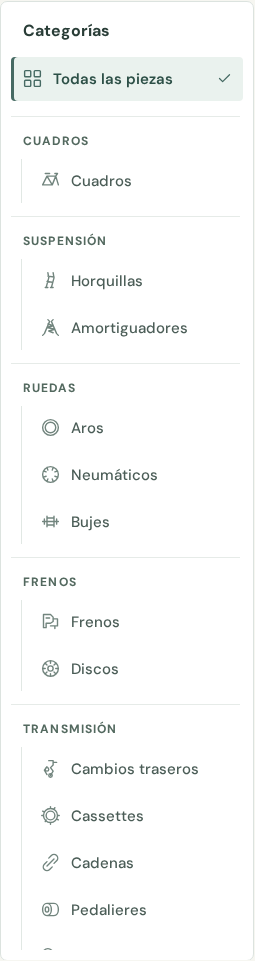
\includegraphics[width=.36\textwidth,height=.66\textheight,keepaspectratio]{recursos/02-categorias.png}
\nota{Captura propia de la aplicación pública. Se muestra el selector para evidenciar agrupación, tamaño de las opciones e iconos, sin destacar nombres comerciales de productos.}
\end{figure}

\subsection{Configuración tridimensional}
La escena se construye con recursos importados y geometría generada por código. GLB es la representación binaria de glTF y permite empaquetar información de una escena para su transmisión \citep{gltf}. En el proyecto se utiliza para recursos reconstruidos y versionados; otros componentes se dibujan a partir de parámetros. Que una pieza sea generada por código no implica que sus datos comerciales se encuentren fuera del catálogo.

Cada recurso incluye un manifiesto con unidades, origen y anclajes de montaje. Las reglas de ensamblaje utilizan esas referencias para colocar piezas respecto del cuadro y de los otros componentes. Se conservan las proporciones y las medidas comerciales registradas, pero las superficies exteriores y ciertos mecanismos se aproximan a partir de referencias. El usuario puede rotar la escena, cambiar vistas, seleccionar una pieza y sustituirla desde el panel correspondiente.

El montaje contempla 23 posiciones. Los pares delantero/trasero pueden aplicarse de forma conjunta cuando existe una alternativa equivalente; si falta la contraparte, la operación no cambia parcialmente la configuración. Los avisos mecánicos distinguen incompatibilidades identificadas de información insuficiente y no convierten la representación en una aprobación de instalación. La inspección de suspensión modifica una postura temporal y se restablece sin reescribir el archivo ni el estado guardado.

\begin{figure}[H]
\caption{Representación tridimensional de un montaje de referencia}\label{fig:montaje}
\centering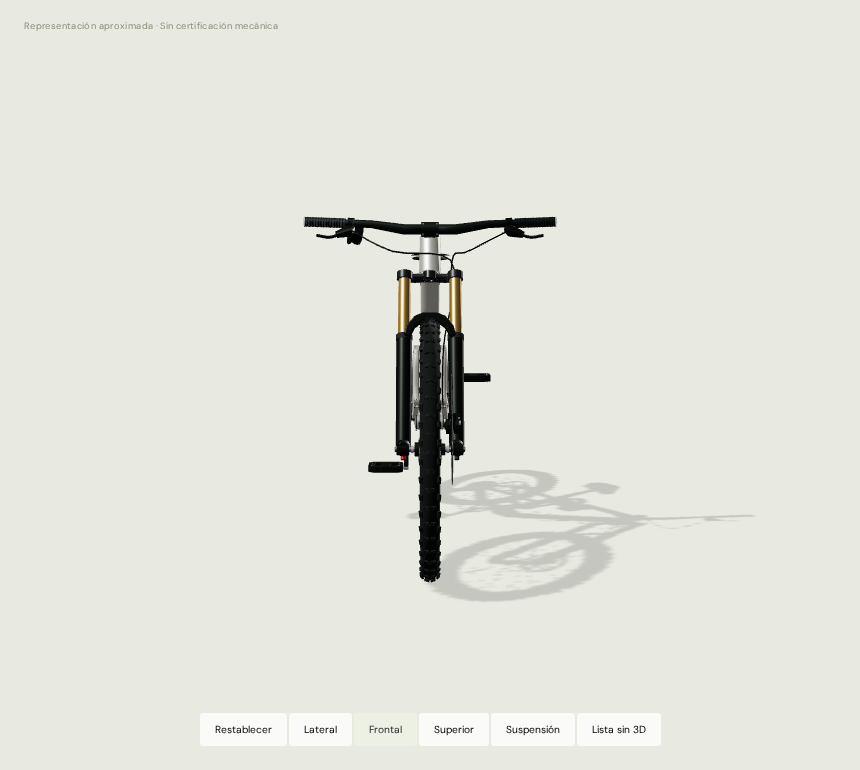
\includegraphics[width=.85\textwidth,height=.55\textheight,keepaspectratio]{recursos/03-montaje-3d.png}
\nota{Captura propia de una sesión temporal de validación. La vista frontal evita destacar rotulación comercial. Se muestra una representación aproximada, no un modelo de fabricación ni una validación mecánica.}
\end{figure}

\subsection{Acceso y gestión de la cuenta}
La aplicación dispone de formularios de credenciales y de acceso con Google. El cliente procesa el retorno autorizado, verifica el código una vez y consulta permisos antes de continuar la intención interna. La cuenta del proveedor no determina un rol administrativo. El menú de cuenta informa identidad y rol, ofrece destinos autorizados y reutiliza el cierre de sesión con aviso de cambios pendientes.

La publicación se realizó en \url{https://atlasmtb.netlify.app/}. Se verificó la configuración del retorno público y la conservación del retorno local de desarrollo. El autor confirmó el acceso real con Google. En cambio, las pruebas con cuentas creadas por API para verificar persistencia no se presentan como evidencia de entrega de correos de confirmación o recuperación. Son procedimientos diferentes y deben conservar esa distinción.

\subsection{Persistencia, versiones y miniaturas}
Guardar envía una configuración validada a una operación transaccional. La cuenta autenticada determina el propietario; la revisión esperada detecta que otra sesión haya actualizado el montaje. Si la revisión es obsoleta, el backend rechaza la escritura y evita reemplazar silenciosamente la versión vigente. La validación pública del informe comprobó ese rechazo con una cuenta temporal.

El catálogo conserva recursos históricos. La auditoría de Storage revisó 316 archivos 3D y encontró 87 usados por las elecciones actuales y 229 históricos. Las huellas y tamaños registrados coincidieron con las copias locales contrastadas; no se detectaron copias idénticas repetidas en esa revisión. Las rutas históricas no se eliminan solo por tener nombres similares, porque los montajes guardados pueden depender de ellas.

Las miniaturas se almacenan separadas del modelo de datos del montaje. Cada imagen corresponde a una revisión visual y se consulta con autorización cuando pertenece a una cuenta. Los recursos GLB públicos facilitan la representación del catálogo; los montajes propios y sus miniaturas no se convierten por ello en información pública.

\subsection{Administración y protección de operaciones}
La interfaz administrativa contiene usuarios, roles y permisos, además de mantenimiento de catálogo y composiciones de referencia. Las cuentas se gestionan mediante una función remota que verifica identidad y autorización antes de utilizar privilegios administrativos. Las operaciones de negocio se expresan en funciones SQL con contratos y comprobaciones de publicación.

El dominio del frontend se añadió a los orígenes admitidos por la función de cuentas. Una comprobación posterior obtuvo autorización de preflight para el dominio público y el local, rechazo para un origen ajeno y rechazo de una petición administrativa sin sesión. Admitir un origen permite la comunicación del navegador, pero no reemplaza la autenticación ni concede permisos de negocio.

\subsection{Publicación y ejecución}
Netlify compila el frontend a partir del repositorio conectado y publica la carpeta de salida. La configuración utiliza \ruta{pnpm run build}, directorio \ruta{dist} y una reescritura de rutas hacia \ruta{index.html}. La documentación del servicio distingue el proceso de compilación y el directorio publicado \citep{netlify}. La aplicación utiliza direcciones de retorno acordes con el origen público.

Las variables públicas identifican el proyecto de Supabase y su clave publicable. Las claves privilegiadas, conexión SQL y credenciales de gestión permanecen fuera del navegador y de los documentos de entrega. La publicación del frontend no despliega automáticamente migraciones o funciones del backend; sus fuentes y procedimientos se mantienen separados.

% Fin: 04-implementacion.tex

\pagina

% Inicio: 05-pruebas-resultados.tex
\section{Pruebas y resultados}
\subsection{Estrategia de validación}
La evaluación se organiza en cuatro niveles: reglas y contratos automatizados; restricciones y operaciones del backend; recorridos de navegador; y comprobación del despliegue público. Cada nivel responde una pregunta distinta. Una prueba de una regla no demuestra que una imagen se entregue por red, y una página que responde HTTP 200 no demuestra que un usuario pueda guardar un montaje.

Vitest permite ejecutar pruebas de código y Playwright automatiza interacciones de navegador \citep{vitest,playwright}. En este proyecto, las pruebas comprueban resultados observables, estados y restricciones. Las capturas del informe documentan la interfaz y no sustituyen las aserciones de guardado, propiedad o revisión.

Para la revisión del informe se ejecutó la suite actual. Una primera pasada produjo un timeout de cinco segundos en una prueba de alineación de componentes bajo concurrencia. Se repitió la suite con dos trabajadores y un límite de quince segundos por prueba, sin cambiar las aserciones ni el código de producto: se obtuvieron 487 pruebas correctas y dos omitidas, distribuidas en 71 archivos correctos y un archivo omitido. El cambio de límite del runner no se interpreta como cumplimiento de una meta de rendimiento del usuario.

\subsection{Validación pública con cuentas temporales}
La comprobación pública utilizó el frontend real de Netlify y dos cuentas temporales creadas y confirmadas por API exclusivamente para la prueba. No se utilizaron datos personales ni contraseñas del autor. La primera cuenta abrió una composición, guardó sus 23 posiciones y volvió a abrirla; la segunda intentó consultar ese montaje. Al finalizar se eliminaron las cuentas y sus recursos temporales. La confirmación por API evita enviar correo y por ello no valida el registro normal por correo electrónico.

\begin{tabla}
\begin{longtable}{L{.9cm}L{4.6cm}L{5.8cm}L{2cm}}
\caption{Matriz de procedimientos y resultados verificados}\label{tab:pruebas}\\\toprule
ID & Procedimiento & Resultado observado & Evidencia\\\midrule\endfirsthead
\multicolumn{4}{l}{\textit{Tabla \thetable\ (continuación)}}\\\toprule ID & Procedimiento & Resultado observado & Evidencia\\\midrule\endhead
T01 & Compilar el frontend & Compilación de TypeScript y salida de Vite correctas. & Registro de build.\\
T02 & Ejecutar reglas y contratos & 487 pruebas correctas, dos omitidas; repetición con dos trabajadores y 15 s de límite. & Registro de Vitest.\\
T03 & Abrir rutas públicas & Portada, catálogo, bicicletas, acceso y callback sirven la aplicación con HTTPS. & HTTP y navegador.\\
T04 & Consultar catálogo y buscar un texto ausente & Se muestran piezas y un estado controlado sin resultados cuando corresponde. & Validación pública.\\
T05 & Autenticar una cuenta temporal & Acceso desde el formulario y apertura del espacio privado. & Navegador real.\\
T06 & Aplicar una composición & La propuesta contiene las 23 posiciones esperadas. & Escena y datos.\\
T07 & Guardar y leer el montaje & Persisten las 23 posiciones y aparece confirmación de guardado. & API de la cuenta.\\
T08 & Consultar con otra cuenta & La consulta del montaje ajeno devuelve cero registros. & Dos identidades.\\
T09 & Guardar con revisión obsoleta & Se rechaza la escritura con código de conflicto PT409. & Operación remota.\\
T10 & Reabrir el montaje guardado & Se abre el detalle de la bicicleta persistida. & Navegador real.\\
T11 & Cerrar sesión & La interfaz vuelve a ofrecer acceso público. & Navegador real.\\
T12 & Revisar móvil emulado & Selector utilizable y ausencia de desbordamiento horizontal a 393 px. & Navegador emulado.\\
T13 & Acceder con Google & Configuración pública leída y recorrido real confirmado por el autor. & Lectura y confirmación manual.\\
T14 & Probar comunicación administrativa & Orígenes público/local admitidos; origen ajeno 403 y visitante 401. & Peticiones al backend.\\
T15 & Abrir y cerrar fichas desde un listado desplazado & Se conserva desplazamiento y foco; salida lateral/móvil y cierre inmediato con movimiento reducido. & Suite de navegador previa.\\\bottomrule
\end{longtable}\end{tabla}
\nota{T15 corresponde a los recorridos de regresión registrados en el proyecto; no se confunde con una medición de teléfono físico. El anexo detalla los archivos de evidencia y las omisiones.}

La validación pública específica registró trece comprobaciones correctas: portada, catálogo, estado sin resultados, entrada, configuración de 23 posiciones, guardado, persistencia, aislamiento, revisión obsoleta, reapertura, cierre, ausencia de errores JavaScript y adaptación móvil emulada. El resumen se conserva como un archivo JSON sin credenciales. Esta comprobación amplía la evidencia del despliegue con operaciones reales y no solo con capturas.

\subsection{Resultados de inventario e infraestructura}
\begin{table}[H]
\caption{Resumen del catálogo e infraestructura en la revisión}\label{tab:snapshot}
\begin{tabla}\begin{tabularx}{\textwidth}{Xr}\toprule
Indicador & Resultado\\\midrule
Modelos publicados & 70\\
Elecciones actuales de variante & 146\\
Variantes conservadas, incluido historial & 782\\
Recursos visuales registrados, incluido historial & 780\\
Composiciones prearmadas públicas & 4\\
Categorías y posiciones de montaje & 18 y 23\\
Tablas propias de negocio y autorización & 8 y 4\\
Migraciones aplicadas & 22\\
Archivos GLB almacenados & 316\\
Archivos GLB usados por elecciones actuales & 87\\
Archivos GLB históricos & 229\\\bottomrule
\end{tabularx}\end{tabla}
\nota{Consultas de lectura del backend y auditoría de archivos. Los recursos visuales incluyen representaciones generadas por código; por ello 780 registros no equivalen a 780 archivos GLB. Las elecciones tampoco equivalen al número de modelos. Elaboración propia.}
\end{table}

La consulta de Storage registró aproximadamente 400 MB de modelos, además de un volumen menor de miniaturas. El frontend compilado observado durante la preparación del despliegue era de aproximadamente 8,8 MB. Esas cifras describen contenido almacenado o publicado y no transferencia mensual. La cantidad de descargas depende del uso, la caché y las piezas consultadas, por lo que no se deduce capacidad de usuarios solo a partir del tamaño de los archivos.

\subsection{Trazabilidad de objetivos}
\begin{table}[H]
\caption{Relación entre objetivos, implementación y evidencia}\label{tab:trazabilidad}
\begin{tabla}\begin{tabularx}{\textwidth}{L{1.5cm}XX}\toprule
Objetivo & Resultado implementado & Evidencia y límite\\\midrule
OE1 & Catálogo estructurado y comparación por categoría & Inventario, pruebas de reglas y recorrido público; sin estudio de comprensión con usuarios.\\
OE2 & Configuración visual y avisos & Montaje de 23 posiciones y escena; aproximación exterior sin certificación mecánica.\\
OE3 & Acceso y persistencia propia & Guardado/reapertura, aislamiento entre cuentas y conflicto de revisión. Correo real pendiente de evaluación específica.\\
OE4 & Administración por permisos & Fuentes, pruebas previas del backend y comprobación pública de rechazo sin sesión; no se reproducen todos los escenarios administrativos en la captura académica.\\
OE5 & Validación y publicación & Suite, recorridos, dominio HTTPS y acceso Google confirmado; móvil físico y resultados de adopción no evaluados.\\\bottomrule
\end{tabularx}\end{tabla}
\nota{Cumplimiento referido a funciones y escenarios comprobados, no a una mejora cuantificada en decisiones de compra. Elaboración propia.}
\end{table}

\subsection{Evidencia visual y adaptación}
La figura~\ref{fig:portada} presenta la entrada pública, y la figura~\ref{fig:movil} muestra la organización del selector en un ancho móvil. Las imágenes se incorporan en el documento y también se entregan como recursos para recompilarlo. No se incluyen capturas de sesiones personales del autor ni paneles con credenciales del backend.

\begin{figure}[H]
\caption{Portada de la aplicación publicada}\label{fig:portada}
\centering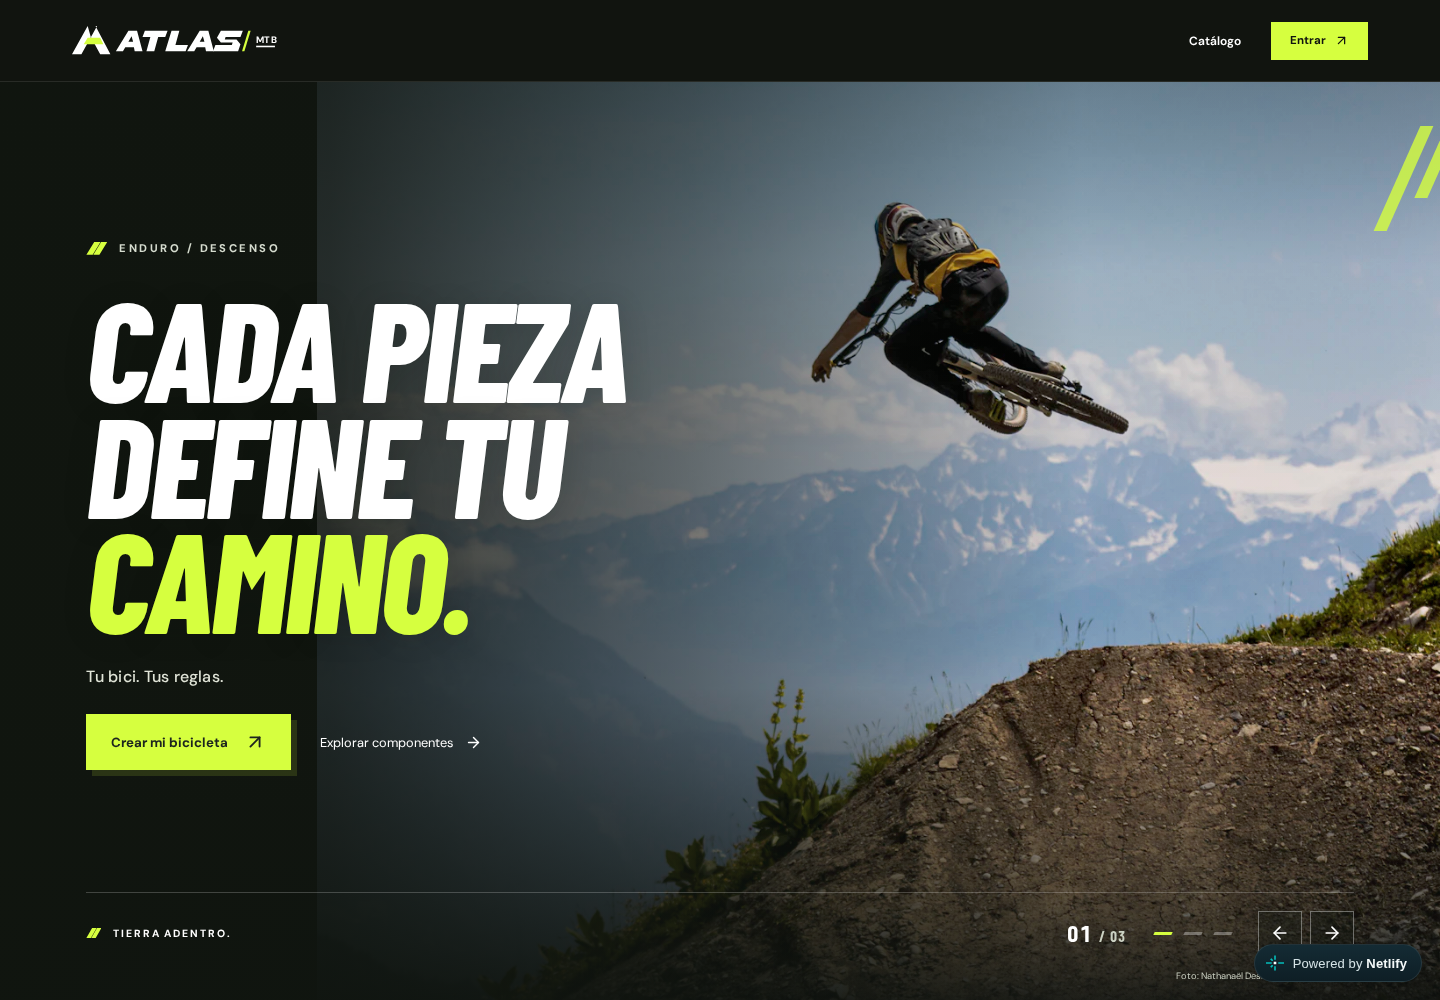
\includegraphics[width=\textwidth,height=.6\textheight,keepaspectratio]{recursos/01-portada.png}
\nota{Captura propia del frontend público. La fotografía de ambientación pertenece a la selección local del proyecto; su procedencia se conserva en el anexo.}
\end{figure}

\begin{figure}[H]
\caption{Selector de categorías en móvil emulado}\label{fig:movil}
\centering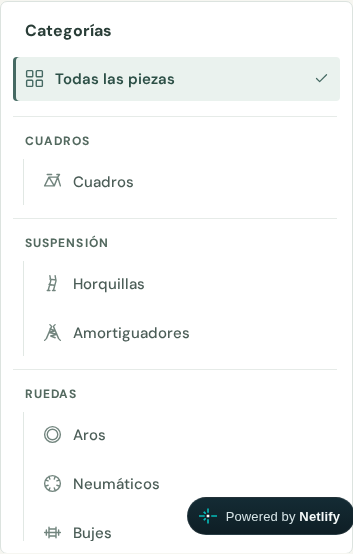
\includegraphics[width=.45\textwidth,height=.6\textheight,keepaspectratio]{recursos/04-categorias-movil.png}
\nota{Captura propia a partir de una ventana de 393 por 851 píxeles. La emulación demuestra disposición e interacción en ese entorno, no rendimiento o funcionamiento de un teléfono físico.}
\end{figure}

\subsection{Dificultades y límites de interpretación}
\begin{enumerate}
\item \textbf{Coherencia de versiones.} Las mejoras de geometría requirieron conservar identidades anteriores y revisar referencias. Una versión más reciente no debe reemplazar silenciosamente las piezas de un montaje existente.
\item \textbf{Interacción y continuidad.} Los cambios de URL de una ficha provocaban restablecimiento del desplazamiento. Se separó la identidad del listado de la identidad del detalle y se añadió cierre visual con restauración de foco sin desplazamiento.
\item \textbf{Configuración de acceso público.} El retorno de autenticación seguía apuntando al entorno local tras publicar. La API de gestión rechazó su actualización con 403, por lo que se guardó desde Dashboard y se comprobó posteriormente por lectura y acceso manual.
\item \textbf{Rendimiento.} La evidencia histórica de una escena de descenso registró 5,454 s bajo una red de prueba de 10 Mbps y 80 ms, frente a un objetivo de 5 s. Mediciones anteriores en renderizado por software estuvieron por debajo de 30 imágenes por segundo. Son resultados de versiones y entornos concretos; no se extrapolan al despliegue actual ni se presentan como metas cumplidas.
\item \textbf{Validación de usuarios.} Las pruebas funcionales no son encuestas de satisfacción ni un ensayo sobre compras. No se dispone de una muestra que permita afirmar reducción de tiempo, ahorro económico o disminución porcentual de errores.
\item \textbf{Correo y dispositivos.} La confirmación de cuentas de prueba por API no valida entrega SMTP. El acceso Google funciona, pero eso no demuestra los flujos completos de correo. La validación móvil utilizada es emulada y no sustituye pruebas en dispositivos físicos.
\end{enumerate}

% Fin: 05-pruebas-resultados.tex

\pagina

% Inicio: 06-conclusiones.tex
\section{Conclusiones y oportunidades de mejora}
\subsection{Conclusiones vinculadas con los objetivos}
\begin{enumerate}
\item Se desarrolló una plataforma que integra consulta, comparación y configuración visual de componentes en un mismo recorrido. El catálogo distingue modelos, variantes y recursos, con 70 modelos y 146 elecciones actuales en la revisión. Esto responde al objetivo de organizar información para evaluar alternativas; no demuestra por sí solo que una población de usuarios comprenda mejor sus decisiones.
\item El configurador permite construir una propuesta de 23 posiciones, sustituir piezas y conservar acabados habilitados. La escena ofrece una representación exterior aproximada y los avisos comunican conflictos conocidos o información insuficiente. El resultado apoya la planificación visual, sin certificar instalación mecánica, resistencia ni recorrido completo de suspensión.
\item La persistencia se comprobó sobre el frontend publicado con cuentas temporales: se guardó y reabrió un montaje completo, otra identidad no pudo leerlo y se rechazó una escritura con revisión obsoleta. Estas evidencias respaldan los escenarios de propiedad e integridad probados, sin sustituir una auditoría completa de seguridad.
\item La administración se implementó mediante permisos explícitos, operaciones de backend y separación de secretos. La publicación requirió ajustar orígenes y direcciones de retorno; las comprobaciones distinguen admisión de comunicación, identidad y autorización. La existencia de una interfaz administrativa no se utilizó como única prueba de protección.
\item El frontend se encuentra disponible con HTTPS en Netlify y mantiene Supabase Cloud como backend. La suite revisada obtuvo 487 pruebas correctas y dos omitidas bajo un runner de concurrencia limitada. El acceso Google fue confirmado por el autor y la revisión pública añadió trece comprobaciones de funcionamiento. Los resultados se presentan con su entorno, alcance y límites.
\end{enumerate}

\subsection{Aprendizajes de gestión y desarrollo}
La experiencia muestra la utilidad de definir criterios de terminación por comportamiento completo: seleccionar, aplicar, guardar y recuperar. Una revisión visual aislada puede ocultar problemas de continuidad, propiedad o estado, mientras una prueba puramente de datos puede omitir fallos de interacción. Mantener reglas separadas de la escena facilitó comprobar decisiones; conservar fuentes y versiones permitió corregir recursos sin invalidar montajes anteriores.

La reconstrucción del cronograma ayuda a explicar dependencias y solapamientos, pero no reemplaza un registro real de dedicación. Para proyectos posteriores conviene registrar desde el inicio fechas efectivas, esfuerzo y cambios de alcance. El trabajo individual también exige reservar tiempo para integración y revisión; concentrar todas las pruebas al final aumenta la incertidumbre del cierre.

\subsection{Oportunidades de mejora}
\begin{enumerate}
\item \textbf{Validación con usuarios.} Evaluar tareas reales con ciclistas y registrar comprensión de variantes, recuperación del montaje y dificultad percibida. Cualquier afirmación de ahorro o mejora debe basarse en un procedimiento y muestra definidos.
\item \textbf{Dispositivos físicos y rendimiento.} Medir carga, memoria y fluidez en teléfonos reales y redes representativas. Utilizar versiones y condiciones identificables para comparar optimizaciones, sin equiparar renderizado por software con desempeño del equipo final.
\item \textbf{Mantenimiento del catálogo.} Establecer una revisión periódica de fuentes, medidas y disponibilidad de variantes, conservando referencias históricas y controles de publicación.
\item \textbf{Flujos de correo.} Configurar y verificar entrega real de confirmación, invitación y recuperación antes de afirmar su aceptación integral. El acceso con un proveedor externo no elimina esa comprobación si se mantiene el registro por correo.
\item \textbf{Accesibilidad y estabilidad.} Ampliar la evaluación con tecnologías de asistencia, errores de red y tareas prolongadas, además de las revisiones actuales de foco, teclado y movimiento reducido.
\item \textbf{Seguimiento operativo.} Revisar cuotas de almacenamiento y transferencia según tráfico observado, y comprobar despliegues posteriores mediante una selección estable de pruebas. No se propone infraestructura adicional sin evidencia de necesidad.
\end{enumerate}

% Fin: 06-conclusiones.tex

\pagina

% Inicio: referencias.tex
\section*{Referencias}\addcontentsline{toc}{section}{Referencias}
\renewcommand{\bibsection}{}
\begingroup
\setlength{\bibhang}{1.27cm}
\setlength{\bibsep}{0pt}
\begin{thebibliography}{99}
\bibitem[Desmeules(2021)]{foto} Desmeules, N.. (2021, 27 de julio). \textit{Man in black jacket and black helmet riding on motocross dirt bike on mountain during daytime} [Fotografía]. Unsplash. \url{https://unsplash.com/photos/man-in-black-jacket-and-black-helmet-riding-on-motocross-dirt-bike-on-mountain-during-daytime-XpB8y73sEEw}
\bibitem[Khronos 3D Formats Working Group(2021)]{gltf} Khronos 3D Formats Working Group. (2021). \textit{glTF 2.0 specification} (versión 2.0.1). \url{https://registry.khronos.org/glTF/specs/2.0/glTF-2.0.html}
\bibitem[Netlify(s. f.)]{netlify} Netlify. (s. f.). \textit{Vite on Netlify}.  \url{https://docs.netlify.com/build/frameworks/framework-setup-guides/vite/}
\bibitem[Playwright(s. f.)]{playwright} Playwright. (s. f.). \textit{Installation}.  \url{https://playwright.dev/docs/intro}
\bibitem[PostgreSQL Global Development Group(s. f.)]{postgres} PostgreSQL Global Development Group. (s. f.). \textit{Row security policies}. PostgreSQL 17 Documentation. \url{https://www.postgresql.org/docs/17/ddl-rowsecurity.html}
\bibitem[React(s. f.)]{react} React. (s. f.). \textit{Thinking in React}.  \url{https://react.dev/learn/thinking-in-react}
\bibitem[Shimano(s. f.)]{shimano} Shimano. (s. f.). \textit{Compatibility}.  \url{https://productinfo.shimano.com/en/compatibility}
\bibitem[SRAM(s. f.)]{sram} SRAM. (s. f.). \textit{Compatibility map}.  \url{https://www.sram.com/en/service/manuals--documents/compatability-map}
\bibitem[Supabase(s. f.-a)]{rls} Supabase. (s. f.-a). \textit{Row level security}.  \url{https://supabase.com/docs/guides/database/postgres/row-level-security}
\bibitem[Supabase(s. f.-b)]{oauth} Supabase. (s. f.-b). \textit{Sign in with Google}.  \url{https://supabase.com/docs/guides/auth/social-login/auth-google}
\bibitem[Vitest(s. f.)]{vitest} Vitest. (s. f.). \textit{Getting started}.  \url{https://vitest.dev/guide/}
\bibitem[World Wide Web Consortium(2024)]{wcag} World Wide Web Consortium. (2024, 12 de diciembre). \textit{Web Content Accessibility Guidelines (WCAG) 2.2}. \url{https://www.w3.org/TR/2024/REC-WCAG22-20241212/}
\end{thebibliography}
\endgroup

% Fin: referencias.tex

\pagina
\appendix

% Inicio: anexos.tex
\section{Diccionario resumido de datos}
Las siguientes tablas identifican entidades y claves relevantes para reconstruir el diseño. El detalle ejecutable se conserva en las migraciones SQL del software. PK significa clave primaria y FK significa clave foránea; no se incluyen datos personales ni valores de conexión.
\begin{tabla}
\begin{longtable}{L{3.5cm}L{5.3cm}L{4.8cm}}
\caption{Entidades de negocio, claves y campos representativos}\label{tab:diccionario}\\\toprule
Entidad & Identidad y relaciones & Campos representativos\\\midrule\endfirsthead
\multicolumn{3}{l}{\textit{Tabla \thetable\ (continuación)}}\\\toprule Entidad & Identidad y relaciones & Campos representativos\\\midrule\endhead
\ruta{brands} & PK id & name, slug, published.\\
\ruta{components} & PK id; FK brand\_id & category, disciplines, description, sources.\\
\ruta{visual_assets} & PK id & kind, storage\_path o generator\_key, manifest.\\
\ruta{component_variants} & PK id; FK component\_id y visual\_asset\_id & label, generation, specs, allowed\_finishes, selectable.\\
\ruta{bike_presets} & PK id; FK brand\_id & family\_key, label, kind, published.\\
\ruta{bike_preset_items} & PK id; FK preset\_id y variant\_id & slot, finish\_id, custom\_color.\\
\ruta{builds} & PK id; FK user\_id a Auth & name, schema\_version, revision, updated\_at.\\
\ruta{build_items} & PK id; FK build\_id y variant\_id & slot, finish\_id, custom\_color.\\\bottomrule
\end{longtable}\end{tabla}

\begin{table}[H]
\caption{Entidades del esquema de autorización}\label{tab:diccionarioiam}
\begin{tabla}\begin{tabularx}{\textwidth}{L{3.7cm}X}\toprule
Entidad & Relación y propósito\\\midrule
\ruta{iam.roles} & PK id; identifica rol, nombre, estado y protección de roles base.\\
\ruta{iam.permissions} & PK code; identifica acciones implementadas y área.\\
\ruta{iam.role_permissions} & PK compuesta role\_id y permission\_code; vincula rol con acciones.\\
\ruta{iam.user_roles} & PK user\_id; FK a identidad y rol; registra revisión de la asignación.\\\bottomrule
\end{tabularx}\end{tabla}
\nota{Las contraseñas no se almacenan en tablas propias. Auth gestiona la identidad y el esquema iam aplica autorización de la aplicación.}
\end{table}

\section{Evidencias, reproducción y procedencia}
\begin{table}[H]
\caption{Archivos de evidencia incluidos con el informe}\label{tab:evidencias}
\begin{tabla}\begin{tabularx}{\textwidth}{L{5.2cm}X}\toprule
Archivo o ubicación & Contenido y alcance\\\midrule
\ruta{recursos/01-portada.png} & Captura de entrada pública con la fotografía ya incorporada a la aplicación.\\
\ruta{recursos/02-categorias.png} & Selector de escritorio, sin destacar modelos comerciales.\\
\ruta{recursos/03-montaje-3d.png} & Escena de una propuesta completa desde cuenta temporal.\\
\ruta{recursos/04-categorias-movil.png} & Selector en viewport móvil emulado.\\
\ruta{recursos/catalogo-resumen.json} & Conteos agregados de lectura: sin cuentas, credenciales o montajes personales.\\
\ruta{recursos/validacion-publica.json} & Trece comprobaciones públicas y confirmación de limpieza de temporales.\\
\ruta{recursos/pruebas-resumen.txt} & Resultado de suite, timeout inicial y condiciones de repetición.\\
\ruta{recursos/compilacion-resumen.txt} & Resultado de compilación del software en la revisión.\\
\ruta{scripts/capture-report-evidence.mjs} & En el software: procedimiento de captura con cuentas temporales y limpieza.\\\bottomrule
\end{tabularx}\end{tabla}
\nota{Las evidencias de cuentas se limitan a resultados agregados. Las capturas no contienen contraseñas, tokens ni correos personales del autor.}
\end{table}

\subsection{Procedimiento de revisión funcional}
Para repetir la comprobación desde el software se instala el entorno declarado y se ejecuta la compilación y la suite. El comando de revisión utilizado para limitar concurrencia fue \ruta{pnpm exec vitest run --maxWorkers=2 --testTimeout=15000}. El parámetro modifica la espera de pruebas, no los requisitos del producto. La evidencia pública puede regenerarse con el script indicado utilizando configuración privada fuera del documento; el procedimiento crea únicamente cuentas temporales y las elimina al terminar.

Las cuentas de prueba se confirman por API administrativa para evitar depender de entrega de correo. El procedimiento no revela sus claves, no modifica el catálogo y comprueba que la lectura de un montaje por otra cuenta no devuelva registros. El archivo de validación identifica los resultados sin incluir la sesión ni datos de conexión. Las pruebas de escritorio y móvil corresponden a navegador Chromium, con vista móvil emulada.

\subsection{Procedencia de imágenes}
Las capturas son elaboración propia a partir del frontend publicado. La fotografía visible en la portada procede de la selección local de ambientación del proyecto. La primera imagen de esa selección es de Nathanaël Desmeules y muestra un salto en Leysin; su página original y licencia se conservan en el archivo de procedencia del software \ruta{src/assets/images/landing/README.md}. La captura reproduce esa interfaz y no atribuye al autor del informe la fotografía original. Se incluye su referencia \citep{foto}.

Los diagramas de arquitectura, relaciones, flujo y Gantt se elaboraron para este informe con código TikZ/pgfgantt, entregado como fuente. No utilizan logotipos institucionales o de proveedores. En la captura del visor se elige una vista frontal para no destacar rotulación de productos; el texto describe las categorías de piezas de manera genérica. Los nombres de tecnologías y autores de las fuentes se identifican cuando son necesarios para que la explicación y las referencias sean verificables.

\section{Correspondencia con la consigna académica}
\begin{table}[H]
\caption{Cobertura del contenido solicitado para el informe}\label{tab:consigna}
\begin{tabla}\begin{tabularx}{\textwidth}{L{5.7cm}X}\toprule
Contenido de la consigna & Ubicación en este informe\\\midrule
Nombre, problemática, justificación y objetivos & Sección 1.\\
Alcance, entregables, cronograma, recursos, responsables y riesgos & Secciones 1 y 2; tabla detallada y Gantt.\\
Requisitos, arquitectura, base de datos y diagramas & Sección 3 y anexo A.\\
Tecnologías, módulos y funcionalidades & Sección 4.\\
Procedimientos, resultados y evidencias & Sección 5 y anexo B.\\
Cumplimiento de objetivos, dificultades y mejoras & Secciones 5 y 6.\\
Fuente LaTeX, recursos y PDF & Carpeta autocontenida 02\_Informe\_Tecnico.\\\bottomrule
\end{tabularx}\end{tabla}
\nota{La modalidad se interpreta como individual según la confirmación del autor. El manual de usuario, la presentación y el software son entregables independientes y no se sustituyen por este informe.}
\end{table}

% Fin: anexos.tex

\end{document}
